\documentclass[a4paper,12pt,onecolumn,twoside]{article}
\usepackage{cite}%bibTeX引用
\usepackage{ctex}
\usepackage{hyperref}%加入超链接
\usepackage{comment}
\usepackage{wrapfig}
\usepackage{graphicx}
\usepackage{float} 
\usepackage{amsmath}
\usepackage{amssymb}
\usepackage{geometry}
\geometry{a4paper,scale=0.8}
\usepackage{float}
\usepackage{subfigure} 
\usepackage{enumerate}%\item 需要
\usepackage{tabularx}% \table 
\usepackage{booktabs}% 	\toprule
\usepackage{longtable}
\usepackage{diagbox}
%%带颜色的表格%%
%\usepackage[table]{xcolor}
\usepackage{colortbl}
\definecolor{mygray}{gray}{.9}
\definecolor{mypink}{rgb}{.99,.91,.95}
\definecolor{mycyan}{cmyk}{.3,0,0,0}
%%带颜色的表格%%
%%附录代码显示%%
\usepackage{listings}

%%附录代码显示%%
%opening

\begin{document}
\begin{center}
	\Large\heiti{天气预报准确度评价}\\
\end{center}
\begin{abstract}
	本文研究了天气预报结果准确度的评价问题,使用可靠性图和Brier技巧评分来评估四种预报的预报效果,得出结论:预报A与预报B的预报效果差,而预报C和预报D的预报效果较为良好,其中预报D优于预报C。\\
	\text{\heiti{关键字:}}天气预报;评价模型;Brier技巧评分
\end{abstract}

\section{问题提出}
\subsection{背景}
明天是否下雨的天气预报以有雨概率形式给出。已得到某地一个月四种预报方法的有雨概率预报,和实际上有雨或无雨的观测结果。根据这四种预报的预报结果,评价它们预报的效果。
\subsection{原始数据}
\begin{longtable}{cccccc} 
		\hline
		日期 & 预报A(\%) & 预报B(\%) & 预报C(\%) & 预报D(\%) & 实测  \\ 
		\hline
		1  & 90      & 30      & 90      & 60      & 1   \\
		2  & 40      & 30      & 50      & 80      & 1   \\
		3  & 60      & 30      & 80      & 70      & 1   \\
		4  & 60      & 30      & 90      & 70      & 1   \\
		5  & 60      & 30      & 0       & 20      & 0   \\
		6  & 30      & 30      & 10      & 50      & 1   \\
		7  & 80      & 30      & 10      & 40      & 0   \\
		8  & 70      & 30      & 20      & 30      & 0   \\
		9  & 80      & 30      & 40      & 30      & 0   \\
		10 & 60      & 30      & 60      & 40      & 0   \\
		11 & 80      & 30      & 20      & 30      & 1   \\
		12 & 40      & 30      & 30      & 40      & 0   \\
		13 & 90      & 30      & 90      & 40      & 1   \\
		14 & 50      & 30      & 60      & 20      & 0   \\
		15 & 10      & 30      & 20      & 10      & 0   \\
		16 & 60      & 30      & 50      & 80      & 1   \\
		17 & 20      & 30      & 10      & 30      & 0   \\
		\hline
		\hline
		日期 & 预报A(\%) & 预报B(\%) & 预报C(\%) & 预报D(\%) & 实测  \\ 
		\hline
		18 & 0       & 30      & 0       & 50      & 0   \\
		19 & 90      & 30      & 60      & 40      & 0   \\
		20 & 70      & 30      & 10      & 0       & 0   \\
		21 & 20      & 30      & 0       & 30      & 0   \\
		22 & 40      & 30      & 20      & 30      & 0   \\
		23 & 40      & 30      & 10      & 10      & 0   \\
		24 & 80      & 30      & 50      & 40      & 0   \\
		25 & 30      & 30      & 0       & 20      & 0   \\
		26 & 30      & 30      & 10      & 30      & 0   \\
		27 & 30      & 30      & 20      & 0       & 0   \\
		28 & 0       & 30      & 60      & 40      & 1   \\
		29 & 60      & 30      & 0       & 20      & 0   \\
		30 & 20      & 30      & 10      & 10      & 0   \\
		31 & 80      & 30      & 50      & 10      & 0   \\
		\hline
\end{longtable}

\section{问题分析}
天气预报给出降雨与否的发生概率在0到1之间,一般来说很难验证单次的预报是否准确,但对于连续的一组预报与实测数据,则可以通过以下三个评判标准来评价其准确程度。
\paragraph{预报者本身的一致性}
该标准指预报者所具备的信息、知识(在本问题中,为气象台测定的数据和其数值预报算法)和其作出的预报之间的关系。倘若气象台没有充分利用测定的信息,亦或者是气象台出于预报效益的考量,人工修改了预报的结果,则认为它的一致性是较差的。例如,依照生活经验,比起预报下雨却没下雨,预报晴天却下雨造成的危害显然是更大的,那么极荒谬的情况下,一个气象台可以次次都预报有雨,如果没有下雨的话也不会造成什么损失,而正巧下雨了的话,预报的订阅者还会认为预报是准确的。\par
本题中的预报B很有可能就是采取了类似的策略,其所有日期的降雨预测均为30\%. 然而,这只是我们作为预报订阅者的一个恶意推断,我们并不知道气象台掌握了多少信息,也不知道他们的数值预报算法,更不知道最后预报出来的数字含有多少人工判断的成分。因此,站在第三方的角度建立评价模型,很难从这一标准入手。
\paragraph{预报和实测间的关系}
这一标准是本问题主要关注的。一种处理方式是,构建混淆矩阵,计数分析预报的准确与否。但这种做法的问题在于,丢失了预报概率本身数值包含的信息。假如一天无雨,那么预报60\%有雨和预报100\%,虽然都是预报错误,但错的离谱程度显然是不同的。若考虑预报的数值,一种常见的方法是绘制可靠性图,也可以通过对两组数据的吻合程度进行打分来评估预测效果。本文选择采用Brier评分来评价预报对实测的准确度。
\paragraph{预报的效益和花费}
预报的效益和预报的准确程度相关性极大,涉及到的其他因素相对复杂且与本问题给出数据无关,我们暂不讨论。\par
\section{可靠性图}
首先,为了能够直观地观察预报的准确程度,我们通过MATLAB软件绘制四个预报结果对实测情况的可靠性图。
\begin{figure}[H]
	\centering
	\subfigure[预报A]{
		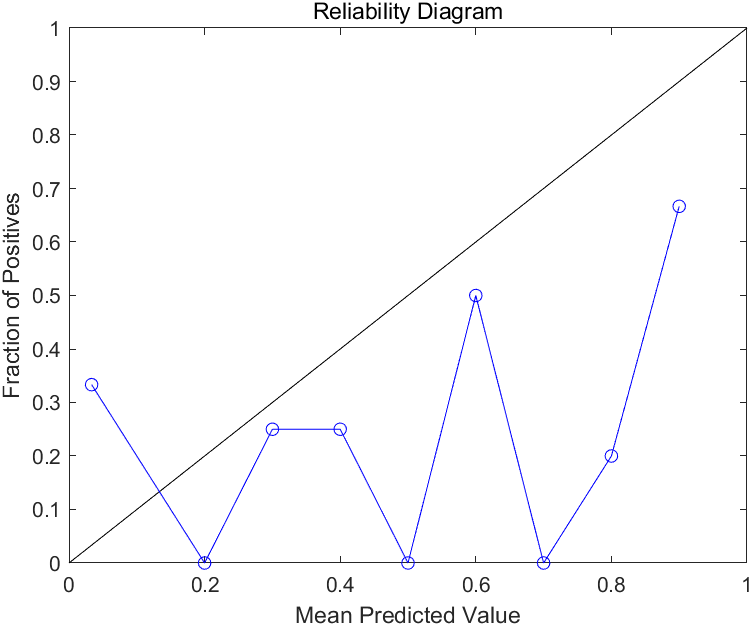
\includegraphics[scale=0.5]{pre1.png} 
	}
	\quad
	\subfigure[预报B]{
		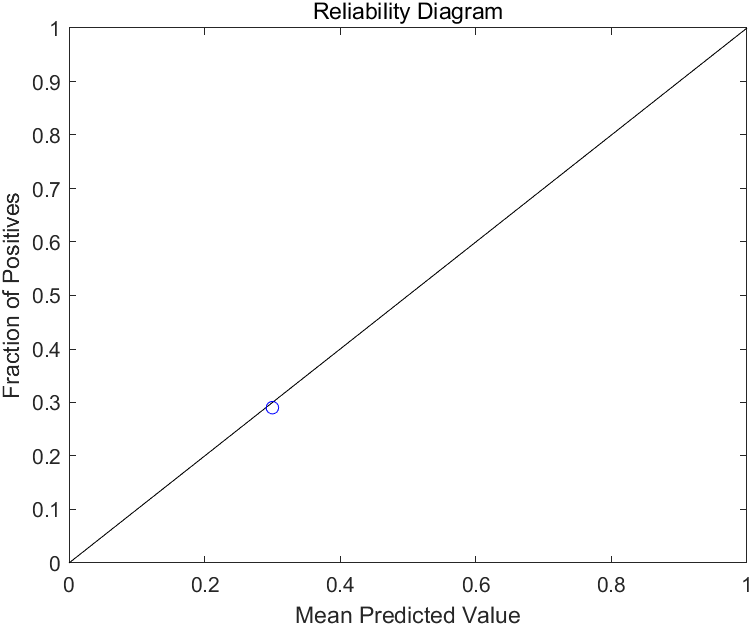
\includegraphics[scale=0.5]{pre2.png} 
	}
	\quad
	\subfigure[预报C]{
		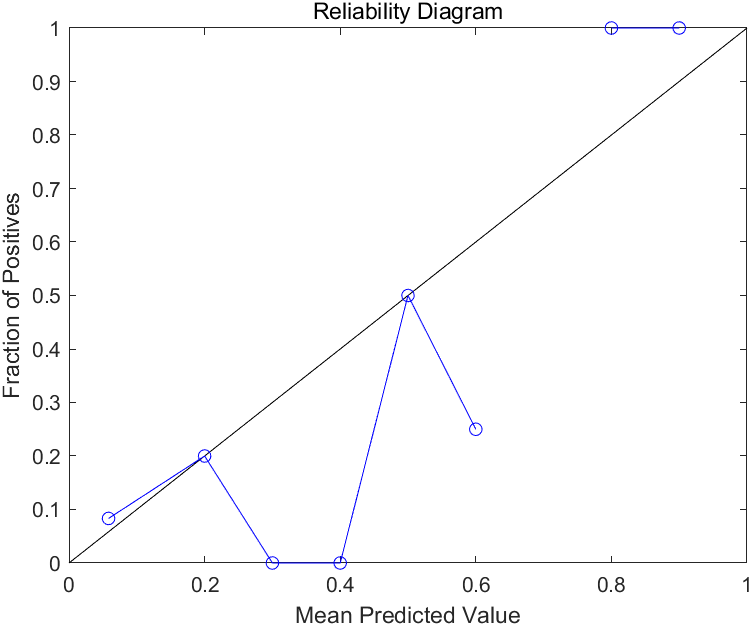
\includegraphics[scale=0.5]{pre3.png} 
	}
	\quad
	\subfigure[预报D]{
	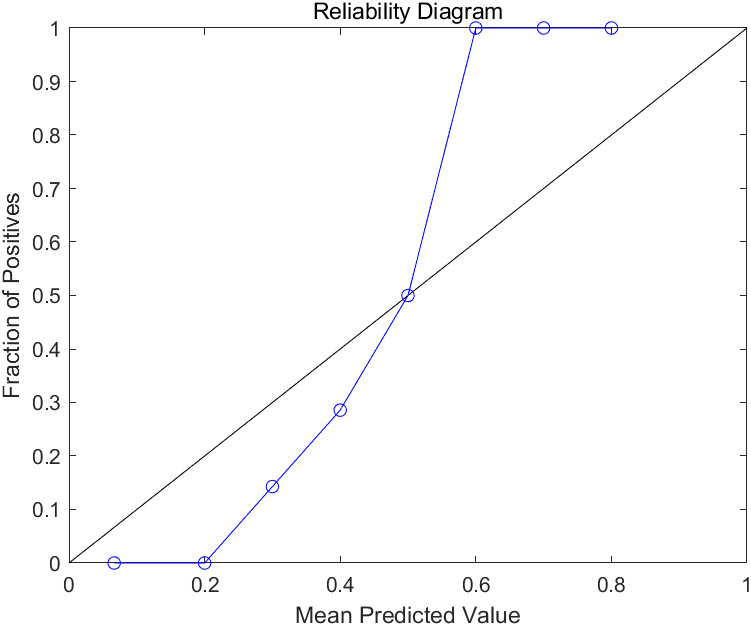
\includegraphics[scale=0.5]{pre4.png} 
	}
	\caption{四个预报的可靠性图}
\end{figure}
其中横坐标为随机变量预测值的概率分布,纵坐标为真实值对预测值的条件概率分布。对角线为预测完全命中观测值的情况,结果越靠近对角线,说明预报越准,如预报C和预报D,这两个预报的可靠性图与对角线趋势较为一致;结果越水平,说明预报越不准,如预报A的情况。\par
但显然,可靠性图无法对预报B的预报结果进行评价,因为预报B取0.3的概率为1,而没有取其他值的情况。此外,对于预报C和预报D,也很难判断孰优孰劣,因此,我们需要借助确切的数值指标来量化预报的准确程度。
\section{Brier评分}
Brier(1950)定义了一种均方概率误差,称为Brier评分,其计算公式为\cite{brier1950verification}
\begin{equation}
	BS=\frac{\sum_{i=1}^{N}(f_{i}-O_{i})^{2}}{N}
\end{equation}
其中,N为预报数,在本题中,为一个月的天数(31);$f_{i}$为第$i$天的预报概率;$O_{i}$为第 $i$ 天的实测结果,若下雨则为1,无雨则为0. $BS$的取值为0-1,且越接近0表示预报效果越好。用MATLAB软件求解,得到四个预报的Brier评分如下表所示。
\begin{table}[H]
	\centering
	\caption{四个预报的Brier评分}
	\begin{tabular}{cc} 
		\hline
		预报 & Brier评分  \\ 
		\hline
		A  & 0.2887   \\
		B  & 0.2061   \\
		C  & 0.1365   \\
		D  & 0.1184   \\
		\hline
	\end{tabular}
\end{table}
Brier评分结果与我们通过可靠性图得出的初步判断是基本一致的,即四个预报中,C和D是较为准确的,且D相较于C更加准确。然而对于B的情况,模型给出的解释是:事件(在本题中为降雨)越罕见,在没有任何实际技能的情况下越容易获得良好的Brier评分。结合本题,在31天中只有9天下雨,那么预报B每一次都预报不下雨(30\%),也可获得较好的Brier评分,而且下雨相对晴天的天数越少,预报B预报的这个概率值越小(例如,每次都预报0\%),它越“歪打正着”。\par
为了避免这种情况,我们再使用Brier技巧评分(Brier Skill score)来评估四个预报的准确性。Brier技巧评分是基于$BS$定义的,它的计算公式为
\begin{equation}
	BSS=\frac{BS-BS_{reference}}{0-BS_{reference}}=1-\frac{BS}{BS_{reference}}
\end{equation}
其中$BS_{reference}$为气候观测值的BS评分,由$BS_{reference}=\bar{O}(1-\bar{O})$计算得到,其中$\bar{O}$为$O_{i}$的期望,可以认为是本月的“平均降雨率”。\par
$BBS$表示预报对“平均降雨率”改进的程度,由式子可以看出,当预报的效果还不如每天都预报“平均降雨率”时,$BBS$的值为负值。因此我们只认为$BBS$为正值的预报是有意义的预报,在这个基础上,$BBS$越大越好,最佳取值为1.\par
四个预报的Brier技巧评分结果如下表所示。
\begin{table}[H]
	\centering
	\caption{四个预报的Brier技巧评分}
	\begin{tabular}{cc} 
		\hline
		预报 & Brier技巧评分  \\ 
		\hline
		A  & -0.4013    \\
		B  & -0.0005    \\
		C  & 0.3377     \\
		D  & 0.4254     \\
		\hline
	\end{tabular}
\end{table}
由表,A和B两预报的效果均被模型认为没有意义,而C与D中,D的预报效果更好。
\section{模型评价}
即便Brier技巧评分对Brier评分作出了一定的改进,它仍然需要大样本来保证模型的稳定性,且事件越罕见,需要的样本越大。


\addcontentsline{toc}{section}{References}
	\bibliographystyle{IEEEtran}
	\bibliography{cite2}
	
\section*{附录:BS, BSS的计算}\addcontentsline{toc}{section}{附录:BS, BSS的计算}
\begin{lstlisting}[language=MATLAB]
%% Brier Score
function [bs] = BS(predict,observed)
% dim predict == dim observed
n=length(predict);
sum=0;
for i = 1:n
count = (predict(i)-observed(i)).^2;
sum = sum+count;
end
bs = sum/n;

%% Brier Skill Score
function [bss] = BSS(predict,observed)
% dim predict == dim observed
obar=mean(observed,"all");
bsref=obar*(1-obar);
bss=1-(BS(predict,observed)./bsref);
end
\end{lstlisting}
\end{document}
